\documentclass[
11pt, % The default document font size, options: 10pt, 11pt, 12pt
%codirector, % Uncomment to add a codirector to the title page
]{charter} 


% El títulos de la memoria, se usa en la carátula y se puede usar el cualquier lugar del documento con el comando \ttitle
\titulo{Mascota interactiva: robot expresivo para la difusión de los posgrados en sistemas embebidos} 

% Nombre del posgrado, se usa en la carátula y se puede usar el cualquier lugar del documento con el comando \degreename
\posgrado{Carrera de Especialización en Sistemas Embebidos} 
%\posgrado{Carrera de Especialización en Internet de las Cosas} 
%\posgrado{Carrera de Especialización en Inteligencia Artificial}
%\posgrado{Maestría en Sistemas Embebidos} 
%\posgrado{Maestría en Internet de las cosas}

% Tu nombre, se puede usar el cualquier lugar del documento con el comando \authorname
% IMPORTANTE: no omitir titulaciones ni tildación en los nombres, también se recomienda escribir los nombres completos (tal cual los tienen en su documento)
\autor{Esp. Ing. Julián Ferreira}

% El nombre del director y co-director, se puede usar el cualquier lugar del documento con el comando \supname y \cosupname y \pertesupname y \pertecosupname
\director{Mg. Ing. Christian Marcelo Yanez Flores}
\pertenenciaDirector{INTI / FIUBA} 
\codirector{Esp. Maria Celeste Corominas} % para que aparezca en la portada se debe descomentar la opción codirector en los parámetros de documentclass
\pertenenciaCoDirector{FIUBA / UNSAM}

% Nombre del cliente, quien va a aprobar los resultados del proyecto, se puede usar con el comando \clientename y \empclientename
\cliente{Nombre del cliente}
\empresaCliente{LSE - FIUBA}
 
\fechaINICIO{20 de octubre de 2026}		%Fecha de inicio de la cursada de GdP \fechaInicioName
\fechaFINALPlan{8 de diciembre de 2026} 	%Fecha de final de cursada de GdP
\fechaFINALTrabajo{31 de agosto de 2027}	%Fecha de defensa pública del trabajo final


\begin{document}

\maketitle
\thispagestyle{empty}
\pagebreak


\thispagestyle{empty}
{\setlength{\parskip}{0pt}
\tableofcontents{}
}
\pagebreak


\section*{Registros de cambios}
\label{sec:registro}


\begin{table}[ht]
\label{tab:registro}
\centering
\begin{tabularx}{\linewidth}{@{}|c|X|c|@{}}
\hline
\rowcolor[HTML]{C0C0C0} 
Revisión & \multicolumn{1}{c|}{\cellcolor[HTML]{C0C0C0}Detalles de los cambios realizados} & Fecha      \\ \hline
0     & Creación del documento                                 	&\fechaInicioName \\ \hline
1	  & Se completa hasta el punto 5 inclusive					& \fechaInicioName \\ \hline
%1      & Se completa hasta el punto 5 inclusive                & {día} de {mes} de 202X \\ \hline
%2      & Se completa hasta el punto 9 inclusive
%		  Se puede agregar algo más \newline
%		  En distintas líneas \newline
%		  Así                                                    & {día} de {mes} de 202X \\ \hline
%3      & Se completa hasta el punto 12 inclusive                & {día} de {mes} de 202X \\ \hline
%4      & Se completa el plan	                                 & {día} de {mes} de 202X \\ \hline

% Si hay más correcciones pasada la versión 4 también se deben especificar acá

\end{tabularx}
\end{table}

\pagebreak



\section*{Acta de constitución del proyecto}
\label{sec:acta}

\begin{flushright}
Buenos Aires, \fechaInicioName
\end{flushright}

\vspace{2cm}

Por medio de la presente se acuerda con el \authorname\hspace{1px} que su Trabajo Final de la \degreename\hspace{1px} se titulará ``\ttitle'' y consistirá en la implementación de un robot expresivo de exhibición, que atraiga visitantes en stands y muestre en vivo cómo funciona por dentro. El trabajo tendrá un presupuesto preliminar estimado de 500 horas y un costo estimado de {\$ 200}, con fecha de inicio el \fechaInicioName\hspace{1px} y fecha de presentación pública el \fechaFinalName.

Se adjunta a esta acta la planificación inicial.

\vfill

% Esta parte se construye sola con la información que hayan cargado en el preámbulo del documento y no debe modificarla
\begin{table}[ht]
\centering
\begin{tabular}{ccc}
\begin{tabular}[c]{@{}c@{}}Dr. Ing. Ariel Lutenberg \\ Director posgrado FIUBA\end{tabular} & \hspace{2cm} & \begin{tabular}[c]{@{}c@{}}\clientename \\ \empclientename \end{tabular} \vspace{2.5cm} \\ 
\multicolumn{3}{c}{\begin{tabular}[c]{@{}c@{}} \supname \\ Director del Trabajo Final\end{tabular}} \vspace{2.5cm} \\
\end{tabular}
\end{table}




\section{1. Descripción técnica-conceptual del proyecto a realizar}
\label{sec:descripcion}

El proyecto consiste en la implementación de un robot expresivo de exhibición, que atraiga visitantes en stands y muestre en vivo cómo funciona por dentro. Se realizará para el Laboratorio de Sistemas Embebidos (LSE) de la Facultad de Ingeniería de la Universidad de Buenos Aires (FIUBA) con el objetivo personal de presentarlo como trabajo final de carrera y lograr la titulación de la carrera Maestría en Inteligencia Artificial Embebida (MIAE) de la FIUBA.

El LSE participará en ferias y eventos para difundir sus posgrados, pero no cuenta con una demostración propia. Los sistemas embebidos son difíciles de mostrar: su funcionamiento no se ve.

La propuesta es una mascota: un robot con una pantalla como cara, que detecta a los visitantes, los sigue con la mirada, cambia de expresión y es capaz de recordar sus nombres. A su lado, un monitor muestra en tiempo real sus tareas, su estado, el tráfico de sus buses y la vista de la cámara con las detecciones e identificaciones de inteligencia artificial. Así el robot atrae al público y el monitor muestra lo que se aprende en la CESE y en la CEIA.

En la figura \ref{fig:diagBloques} se muestra el diagrama de bloques del sistema. Se observa que el controlador principal recibe la información del sensor de presencia y comanda la pantalla, el cuello, el parlante y los LEDs. Además envía telemetría al monitor de la vista por dentro. A través del conector de expansión se vincula con el módulo de inteligencia artificial (CEIA), procesado en el ordenador/placa Linux, y se permite sumar a futuro agregados de IoT sin modificar el diseño base. 

\begin{figure}[htpb]
\centering 
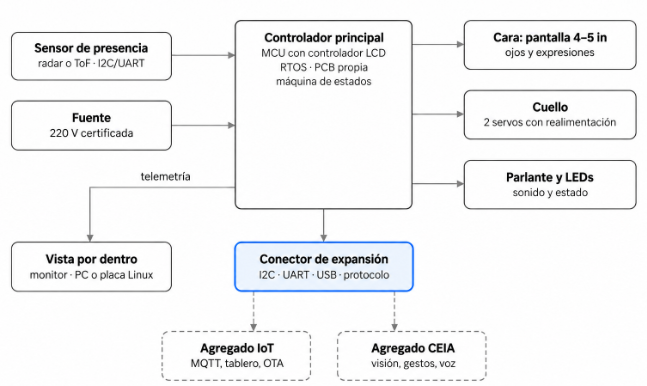
\includegraphics[width=.65\textwidth]{./Figuras/diagBloques.png}
\caption{Diagrama en bloques del sistema.}
\label{fig:diagBloques}
\end{figure}

La figura \ref{fig:ImplementacionFinal} muestra una versión de lo esperado.

\begin{figure}[htpb]
\centering 
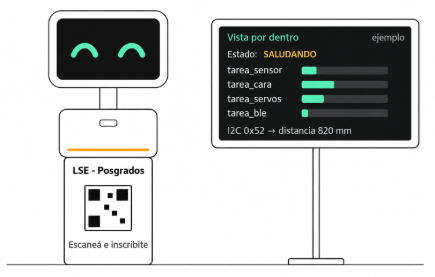
\includegraphics[width=.65\textwidth]{./Figuras/ImplementacionFinal.png}
\caption{Vista de implementación final.}
\label{fig:ImplementacionFinal}
\end{figure}

\vspace{25px}

\section{2. Identificación y análisis de los interesados}
\label{sec:interesados}

\begin{table}[ht]
\caption{Identificación de los interesados}
\label{tab:interesados}
\begin{tabularx}{\linewidth}{|l|>{\raggedright\arraybackslash}X|>{\raggedright\arraybackslash}X|>{\raggedright\arraybackslash}X|}
\hline
\rowcolor[HTML]{C0C0C0} 
Rol           & Nombre y Apellido & Organización    &	Puesto                    \\ \hline
Cliente       & \cosupname        & \empclientename & Coordinadora Académica CEIoT, LSE-FIUBA \\ \hline
Responsable   & \authorname       & FIUBA           & Alumno                    \\ \hline
Orientador    & \supname          & \pertesupname   & Director del Trabajo Final \\ \hline
Usuario final & -                 & \empclientename & Expositores en stands del LSE \\ \hline
\end{tabularx}
\end{table}

\begin{itemize}
	\item Cliente: LSE, es el que va a aprobar los resultados del proyecto.
	\item Orientador: coordinador académico del CESE. Guía referente a la temática de sistemas embebidos del proyecto.
	\item Usuario final: expositores en stands durante distintas ferias de posgrados.
\end{itemize}

\section{3. Propósito del proyecto}
\label{sec:proposito}

El propósito del proyecto es desarrollar un robot expresivo de exhibición, destinado al Laboratorio de Sistemas Embebidos (LSE) de la Facultad de Ingeniería de la Universidad de Buenos Aires (FIUBA), que atraiga visitantes en stands y muestre en vivo cómo funciona por dentro. El valor principal es difundir los posgrados en sistemas embebidos, demostrando de manera interactiva y atractiva lo que se aprende en la Carrera de Especialización en Sistemas Embebidos (CESE) y la Carrera de Especialización en Inteligencia Artificial (CEIA), sin depender de proyectos externos.

\section{4. Alcance del proyecto}
\label{sec:alcance}

Se busca crear un robot expresivo de exhibición, que pueda:

\begin{itemize}
	\item Mover el cuello como lo hace un humano, 180° en torno al eje vertical y 90° en torno al eje horizontal.
	\item Detectar presencia de personas.
	\item Mostrar expresiones faciales en una pantalla, incluyendo ojos y boca. 
	\item Capacidad de interactuar con personas mediante juegos.
	\item Detectar distintos objetos a definir para generar juegos interactivos con las personas. 
	\item Recibir comandos de voz y responder con voz sintetizada.
	\item Mostrar en un monitor externo la telemetría del robot, incluyendo:
		\begin{itemize}
		\item Estado de los sensores.
		\item Visualización de datos.
		\item Estado de los buses de comunicación.
		\item Vista de la cámara con las detecciones e identificaciones de inteligencia artificial.
		\end{itemize}
\end{itemize}

\section{5. Supuestos del proyecto}
\label{sec:supuestos}

Para el desarrollo del presente proyecto se supone que: 

\begin{itemize}
	\item Se dispondrá de al menos 12 horas semanales para realizar avances.
	\item Se contará con USD 200 para la compra de materiales y componentes, provistos por el LSE.
	\item Se cuenta con los materiales necesarios para la construcción de la carcasa del robot, incluyendo impresora 3D y filamento.
	\item Se contará con el apoyo del LSE para la resolución de problemas de hardware y software que puedan surgir durante el desarrollo del proyecto.
	\item Los componentes y materiales necesarios para el desarrollo del proyecto estarán disponibles en el mercado.
	\item Para la generacion del cuerpo del robot se cuenta con el uso de modelos libres. 
\end{itemize}

\section{6. Requerimientos}
\label{sec:requerimientos}

En esta sección se describen los distintos requerimientos establecidos para el proyecto propuesto:

\begin{enumerate}
	\item Requerimientos funcionales:
		\begin{enumerate}
			\item Funcionar durante 8 horas continuas con público y sin intervención.
			\item Detectar a un visitante y orientar la cabeza hacia él en menos de 1 segundo.
			\item Alimentarse mediante la red de 220 V con una fuente certificada.
			\item El robot debe ser capaz de girar su cabeza 180° en torno al eje vertical y 90° en torno al eje horizontal.
			\item Reconocer comandos por voz y tener la capacidad de responder.
		\end{enumerate}
	\item Requerimientos no funcionales:
		\begin{enumerate}
			\item Garantizar la seguridad física evitando partes móviles expuestas que puedan atrapar dedos.
			\item  Permitir el armado y la puesta en marcha en menos de 15 minutos. 
		\end{enumerate}	
	\item Requerimientos de interacción y reconocimiento:
		\begin{enumerate}
			\item Identificar a los visitantes previamente registrados durante la jornada y mostrar sus nombres en el monitor lateral en tiempo real.
			\item Contabilizar la cantidad de personas detectadas frente al stand durante la exhibición.
			\item Ejecutar detección y clasifiacion de objetos especificos a definir.
			\item Capaz de inicar comandos mediante comandoz de vos recibidos. 
			\item Responder cuando un visitante deja el stand con un mensaje de adios usando un modulo de salida de audio. 
		\end{enumerate}
	\item Requerimientos de subsistemas y hardware:
		\begin{enumerate}
			\item El controlador principal debe contar con un controlador LCD implementado en una placa de circuito impreso propia.
			\item El sistema debe operar mediante una máquina de estados para gestionar las expresiones (reposo, saludo, sorpresa, dormido).
			\item Contar con una pantalla de 4 a 5 pulgadas para la animación de ojos y expresiones.
			\item Contar con un cuello de dos ejes con servos con realimentación.
			\item Conectar el sensor de presencia y los subsistemas mediante protocolos como I2C o UART.
			\item Enviar telemetría hacia una PC o placa Linux para visualizar en un monitor lateral las tareas, el estado, el tráfico de los buses y las detecciones de IA en vivo.
		\end{enumerate}
	\item Requerimientos de extensibilidad y arquitectura:
		\begin{enumerate}
			\item Incluir un conector de expansión físico que proporcione alimentación, I2C, UART y USB.
			\item Definir un protocolo de mensajes documentado para el intercambio de comandos y eventos.
			\item Implementar una arquitectura en capas que aísle el hardware de la lógica de comportamiento, permitiendo incorporar futuros agregados de IoT sin alterar el firmware base.
		\end{enumerate}
	\item Requerimientos de calidad:
		\begin{enumerate}
			\item Aplicar capas de abstracción, análisis estático y una batería de tests unitarios y de integración.
		\end{enumerate}
	\item Requerimientos de entregables:
		\begin{enumerate}
			\item Firmware documentado y versionado.
			\item Especificación técnica del conector y protocolo de expansión.
			\item Manual completo de armado, uso y mantenimiento.
		\end{enumerate}
\end{enumerate}

\section{7. Historias de usuarios (\textit{Product backlog})}
\label{sec:backlog}

Las historias de usuario (HU) serán ponderadas utilizando \textit{Story Points}, asignados según el
siguiente criterio:

\begin{itemize}
	\item Dificultad: cantidad de tiempo que lleva la tarea.
		\begin{itemize}
			\item Nivel bajo: 2
			\item Nivel medio: 5
			\item Nivel alto: 13
		\end{itemize}
	\item Complejidad: dificultad para ejecutar la tarea en un corto período de tiempo debido a la
complejidad y desafíos que presenta.
		\begin{itemize}
			\item Nivel bajo: 5
			\item Nivel medio: 13
			\item Nivel alto: 21
		\end{itemize}
	\item Incertidumbre: nivel de riesgo que involucra realizar la tarea según el nivel de conocimiento
previo.
		\begin{itemize}
			\item Nivel bajo: 1
			\item Nivel medio: 5
			\item Nivel alto: 13
		\end{itemize}
\end{itemize}

Sumando el nivel de dificultad, complejidad e incertidumbre, se busca el siguiente valor más
cercano en la serie de Fibonacci y así se obtiene el peso del Story Point.

\begin{itemize}
	\item Como cliente quiero que el robot pueda detectar a un visitante y orientar la cabeza hacia él en menos de un segundo para mostrar que el sistema es dinámico y atractivo.

	\textit{Story Points}: 21 (dificultad: 5, complejidad: 13, incertidumbre: 1)
	\item Como cliente quiero que el sistema pueda armarse y ponerse en marcha en menos de 15 minutos para que su puesta en marcha en distintas exhibiciones sea sencilla.

	\textit{Story Points}: 55 (dificultad: 13, complejidad: 21, incertidumbre: 5)
	\item Como cliente quiero que el sistema pueda detectar rostros de personas en tiempo real para mostrar las enseñanzas que se imparten en la CEIA.

	\textit{Story Points}: 13 (dificultad: 5, complejidad: 5, incertidumbre: 1)
	\item Como cliente quiero que el sistema cuente con una placa de extensión para poder agregar fácilmente a futuro funcionalidades relacionadas a otras carreras del LSE.

	\textit{Story Points}: 55 (dificultad: 13, complejidad: 21, incertidumbre: 13)
	\item Como cliente quiero que el sistema reconozca comandos de voz de visitantes para poder recordar el nombre de la persona y poder mostrar su rostro con su nombre en caso de que pase nuevamente por el stand.

	\textit{Story Points}: 55 (dificultad: 13, complejidad: 13, incertidumbre: 13)
	\item Como cliente quiero que el sistema cuente con una pantalla para mostrar el estado interno del sistema para poder demostrar cómo se está comportando internamente el robot en cada una de sus acciones.

	\textit{Story Points}: 8 (dificultad: 2, complejidad: 5, incertidumbre: 1)
	\item Como cliente quiero que el robot sea capaz de funcionar 8 horas continuas sin intervención, para poder exponer durante una jornada completa el mismo.

	\textit{Story Points}: 8 (dificultad: 2, complejidad: 5, incertidumbre: 1)
	\item Como cliente quiero contar con una documentación completa del firmware y protocolos de comunicación para ayudar a realizar expansiones futuras.

	\textit{Story Points}: 34 (dificultad: 13, complejidad: 13, incertidumbre: 1)
\end{itemize}

\section{8. Entregables principales del proyecto}
\label{sec:entregables}

\begin{itemize}
	\item Memoria del trabajo final.
	\item Robot funcional.
	\item Firmware documentado y versionado, con su batería de tests.
	\item Aplicación de ``vista por dentro'' para el monitor lateral, integrando la visualización de telemetría embebida y el visor de inteligencia artificial en tiempo real.
	\item Especificación del conector y del protocolo de expansión, validado mediante la integración del módulo de reconocimiento facial e interacción (CEIA).
	\item Manual de armado, uso y mantenimiento para el laboratorio.
\end{itemize}

\section{9. Desglose del trabajo en tareas}
\label{sec:wbs}

\begin{enumerate}
\item Investigacion y desgloce macro de diseño (15 h)
	\begin{enumerate}
	\item Investigacion de proyectos indole similar (4 h)
	\item Invesitgacion y Seleccion de pantalla LCD y controlador del mismo (6 h)
	\item Investigacion y seleccion de servomotores (2 h)
	\item Definicion de estetica del robot (3 h)
	\end{enumerate}
\item Eleccion de harware (suma h)
	\begin{enumerate}
	\item Invesitgacion y seleccion de sensores de sercania/deteccion (4 h)
	\item Inestigacion y seleccion modulos de entrada de audio (4 h)
	\item Investigacion y seleccion de modulos de salida de audio (4 h)
	\item Invesitgacion y seleccion de modulo del LCD seleccionado (4 h)
	\item Investigacion y selecccion de un modulo comunicacion conuunta de I2C, UART y USB (4 h)
	\item Inestigacion y seleccion de  modulo o camara pequeña (4 h)
	\item Investigacion  y seleccion de placa de desarrollo a utilzar (8 h)
	\item Definicion de requsitos minimos de computadora externa a utilizar (4 h)
	\end{enumerate}
\item Desarrollo de firwmare (suma h)
	\begin{enumerate}
	\item Definir el diseño del firmware del sistema (3 h)
	\item Generacion de protocolo de comunicacion propio del robot (8 h)
	\item Implemetnacion de driver de pantalla LCD (10 h)
	\item Implemenbtacion de driver de pruebas de pantalla LCD (10 h)
	\item Implementacion de driver de movimiento de servos (4 h)
	\item Implementacion de driver de prueba de movimiento de servos (4 h)
	\item Implementacion de driver de sensores de sercania/deteccion (6 h)
	\item Implementacion de driver prueba de sensores de sercania/deteccion (6 h)
	\item Implementacion de dirver de entrada de audio (6 h)
	\item Implementcion de driver de salida de audio (6 h)
	\end{enumerate}
\item Desarrollo de modulode de IA (suma h)
	\begin{enumerate}
		\item Investigacion y seleccion de modelo pre entrenado de reconomineto de personas (2 h)
		\item Seleccion de objetos para juego interactivo (1 h)
		\item Investigacion y seleccion de modelo preentrenado para deteccion de objetos en base a objetos seleccionados (2 h)
		\item Investigacion y seleccion de modelo preenetrenado de lenguaje humano (2 h)
		\item Desarollo de sistema de reconocimiento de personas (2 h)
		\item Desarrollo de sistema de reconocimiento de objetos (2 h)
		\item Desarrollo de sistema de modelo de lenguaje humano (4 h)
		\item Desarrollo de modulo de software del protocolo de comuniacion propio del robot (2 h)
		\item Desarrollo de software de modulo IA externo del robot (2 h)
		\item Desarrollo de test software de modeulo IA externo del robot (6 h)
	\end{enumerate}
\item Desarrollo inegrado del sistema
	\begin{itemize}
		\item Unificacion de de modulos de Firmware en sistema central (40 h)
		\item Desarrollo de estetica de robot (10 h)
		\item Integracion de modulos de hardware con estetica de robot y primer armado (5 h)
		\item Busqueda de optimizacion de armado (20 h)
		\item Prueba de puesta en marhca y prueba general de hardware (5 h)
		\item Prueba de integracion de harwared e IA (6 h)
		\item Arregñp de bugs o no funcionalidades (20 h)
	\end{itemize}
\item Puesta en marcha
	\begin{itemize}
		\item Segundo armado (4 h)
		\item Prueba de puesta en marcha (5 h)
		\item Prueba de largo tiempo funcionado (12 h)
		\item Prueba de demo de interaccion (2 h)
	\end{itemize}
\item Docuemtnacion de entregables
	\begin{enumerate}
		\item Docuemtnacion de firmwre (10 h)
		\item Manual de puesta en marcha (10 h)
		\item Documentacion de protocols del robot (10 h)
		\item Manual de integracion de nuevo modulos (10 h)
	\end{enumerate}
\item Documentacion trabajo final
	\begin{enumerate}
		\item Redacciona de taller de trabajo final A (30 h)
		\item Redacciona de taller de trabajo final B (30 h)
		\item Presentacion final (1 h)
	\end{enumerate}
\end{enumerate}

Cantidad total de horas: tantas.


\section{10. Diagrama de Activity On Node}
\label{sec:AoN}

\begin{consigna}{red}
Armar el AoN a partir del WBS definido en la etapa anterior.

Una herramienta simple para desarrollar los diagramas es el Draw.io (\url{https://app.diagrams.net/}).
\href{https://app.diagrams.net}{Draw.io}


\begin{figure}[htpb]
\centering 
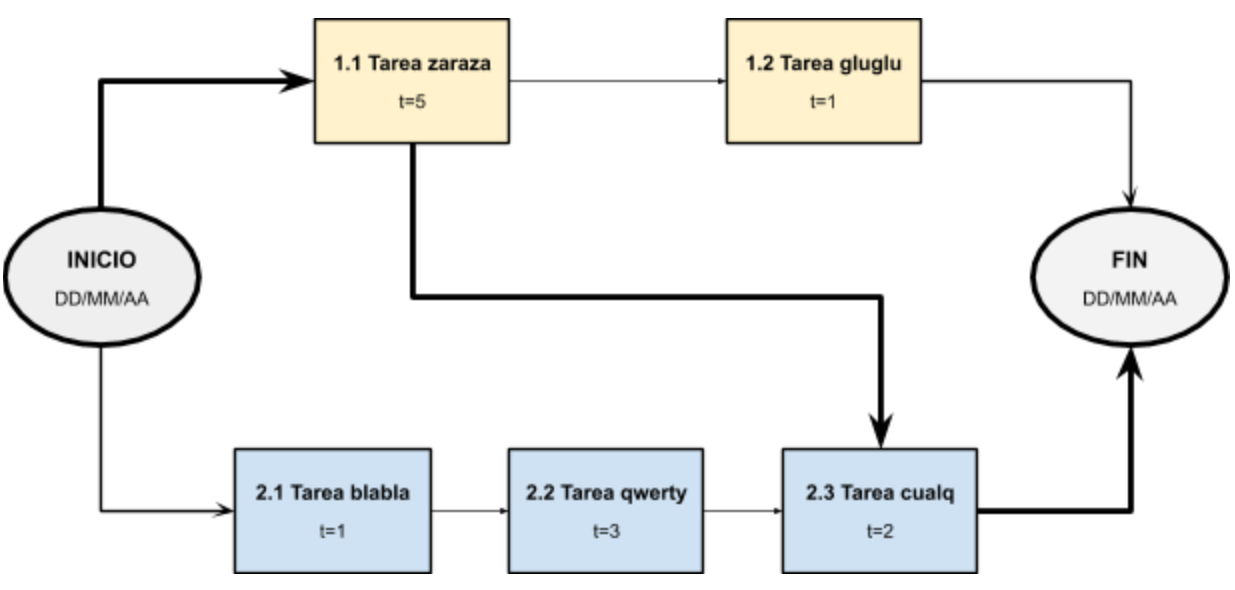
\includegraphics[width=.8\textwidth]{./Figuras/AoN.png}
\caption{Diagrama de \textit{Activity on Node}.}
\label{fig:AoN}
\end{figure}

Indicar claramente en qué unidades están expresados los tiempos.
De ser necesario indicar los caminos semi críticos y analizar sus tiempos mediante un cuadro.
Es recomendable usar colores y un cuadro indicativo describiendo qué representa cada color.

\end{consigna}

\section{11. Diagrama de Gantt}
\label{sec:gantt}

\begin{consigna}{red}
Existen muchos programas y recursos \textit{online} para hacer diagramas de Gantt, entre los cuales destacamos:

\begin{itemize}
\item Planner
\item GanttProject
\item Trello + \textit{plugins}. En el siguiente link hay un tutorial oficial: \\ \url{https://blog.trello.com/es/diagrama-de-gantt-de-un-proyecto}
\item Creately, herramienta online colaborativa. \\\url{https://creately.com/diagram/example/ieb3p3ml/LaTeX}
\item Se puede hacer en latex con el paquete \textit{pgfgantt}\\ \url{http://ctan.dcc.uchile.cl/graphics/pgf/contrib/pgfgantt/pgfgantt.pdf}
\end{itemize}

Pegar acá una captura de pantalla del diagrama de Gantt, cuidando que la letra sea suficientemente grande como para ser legible. 
Si el diagrama queda demasiado ancho, se puede pegar primero la ``tabla'' del Gantt y luego pegar la parte del diagrama de barras del diagrama de Gantt.

Configurar el software para que en la parte de la tabla muestre los códigos del EDT (WBS).\\
Configurar el software para que al lado de cada barra muestre el nombre de cada tarea.\\
Revisar que la fecha de finalización coincida con lo indicado en el Acta Constitutiva.

En la figura \ref{fig:gantt}, se muestra un ejemplo de diagrama de gantt realizado con el paquete de \textit{pgfgantt}. 
En la plantilla pueden ver el código que lo genera y usarlo de base para construir el propio.

Las fechas pueden ser calculadas utilizando alguna de las herramientas antes citadas. Sin embargo, el siguiente ejemplo
fue elaborado utilizando 
\href{https://docs.google.com/spreadsheets/d/1fBz8NhSpc4tkkhz3KjJCbh1nR_ltDkfEcZi4tZXduqs}{esta hoja de cálculo}.

Es importante destacar que el ancho del diagrama estará dado por la longitud del texto utilizado para las tareas 
(Ejemplo: tarea 1, tarea 2, etcétera) y el valor \textit{x unit}. Para mejorar la apariencia del diagrama, es necesario
ajustar este valor y, quizás, acortar los nombres de las tareas.

\begin{figure}[htpb]
  \begin{center}
    \begin{ganttchart}[
      time slot unit=day,
      time slot format=isodate,
      x unit=0.038cm,
      y unit title=0.7cm,
      y unit chart=0.6cm,
      milestone/.append style={xscale=4}
      ]{2021-03-05}{2021-12-16}
      \gantttitlecalendar*{2021-03-05}{2021-12-16}{year} \\
      \gantttitlecalendar*{2021-03-05}{2021-12-16}{month} \\
      \ganttgroup{Duración Total}{2021-03-05}{2021-12-16} \\
      %%%%%%%%%%%%%%%%%Organización
      \ganttgroup{Organización}{2021-03-05}{2021-04-16} \\
      \ganttbar{Planificación del proyecto}{2021-03-05}{2021-04-15} \\
      %%%%%%%%%%%%%%%%%Ejecución
      \ganttgroup{Ejecución}{2021-04-16}{2021-10-21} \\
      \ganttbar{Tarea 1}{2021-04-16}{2021-04-29} \\
      \ganttbar{Tarea 2}{2021-04-30}{2021-05-13} \\
      \ganttbar{Tarea 3}{2021-05-14}{2021-05-27} \\
      \ganttbar{Tarea 4}{2021-05-28}{2021-07-12} \\
      \ganttbar{Tarea 5}{2021-07-13}{2021-08-09} \\
      \ganttbar{Tarea 6}{2021-08-10}{2021-09-23} \\
      \ganttbar{Tarea 7}{2021-09-24}{2021-09-30} \\
      \ganttbar{Tarea 8}{2021-10-01}{2021-10-14} \\
      \ganttbar{Tarea 9}{2021-10-15}{2021-10-21} \\
      % %%%%%%%%%%%%%%%%%Finalización
      \ganttgroup{Finalización}{2021-10-22}{2021-12-16} \\
      \ganttbar{Memoria v1}{2021-10-22}{2021-11-04} \\
      \ganttbar{Memoria v2}{2021-11-05}{2021-11-18} \\
      \ganttbar{Memoria final}{2021-11-19}{2021-12-02} \\
      % La fecha del siguiente milestone es la fecha en que terminamos la memoria
      \ganttmilestone{Enviar memoria al director}{2021-12-02} \\
      \ganttbar{Elaborar la presentación}{2021-12-03}{2021-12-16} \\
      \ganttmilestone{Ensayo de la presentación}{2021-12-16} \\
      %%%%%%%%%%%%%%%%%%%%%%%%%%%%%%%%%%%%%%%%%%%%%%%%%%%%%%%%%%%%%%%
    \end{ganttchart}
  \end{center}
  \caption{Diagrama de gantt de ejemplo}
  \label{fig:gantt}
\end{figure}


\begin{landscape}
\begin{figure}[htpb]
\centering 
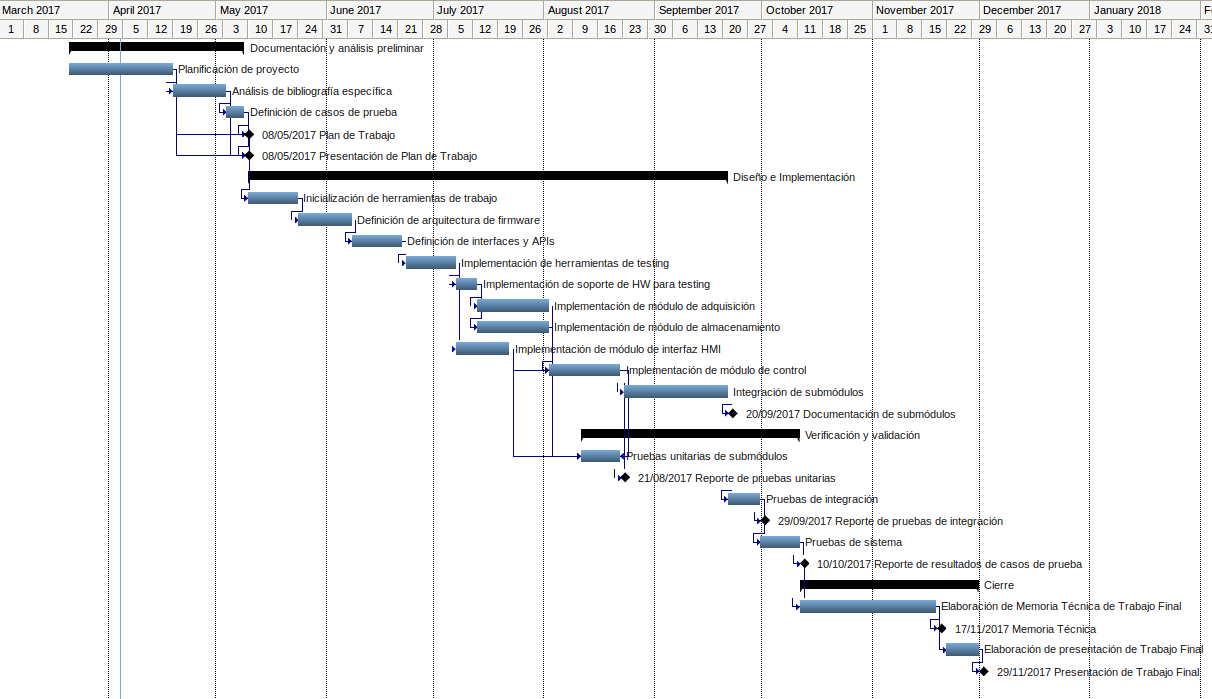
\includegraphics[height=.85\textheight]{./Figuras/Gantt-2.png}
\caption{Ejemplo de diagrama de Gantt (apaisado).} %Modificar este título acorde.
\label{fig:diagGantt}
\end{figure}

\end{landscape}

\end{consigna}


\section{12. Presupuesto detallado del proyecto}
\label{sec:presupuesto}

\begin{consigna}{red}
Si el proyecto es complejo entonces separarlo en partes:
\begin{itemize}
	\item Un total global, indicando el subtotal acumulado por cada una de las áreas.
	\item El desglose detallado del subtotal de cada una de las áreas.
\end{itemize}

IMPORTANTE: No olvidarse de considerar los COSTOS INDIRECTOS.

Incluir la aclaración de si se emplea como moneda el peso argentino (ARS) o si se usa moneda extranjera (USD, EUR, etc). Si es en moneda extranjera se debe indicar la tasa de conversión respecto a la moneda local en una fecha dada.

\end{consigna}

\begin{table}[htpb]
\centering
\begin{tabularx}{\linewidth}{@{}|X|c|r|r|@{}}
\hline
\rowcolor[HTML]{C0C0C0} 
\multicolumn{4}{|c|}{\cellcolor[HTML]{C0C0C0}COSTOS DIRECTOS} \\ \hline
\rowcolor[HTML]{C0C0C0} 
Descripción &
  \multicolumn{1}{c|}{\cellcolor[HTML]{C0C0C0}Cantidad} &
  \multicolumn{1}{c|}{\cellcolor[HTML]{C0C0C0}Valor unitario} &
  \multicolumn{1}{c|}{\cellcolor[HTML]{C0C0C0}Valor total} \\ \hline
 &
  \multicolumn{1}{c|}{} &
  \multicolumn{1}{c|}{} &
  \multicolumn{1}{c|}{} \\ \hline
 &
  \multicolumn{1}{c|}{} &
  \multicolumn{1}{c|}{} &
  \multicolumn{1}{c|}{} \\ \hline
\multicolumn{1}{|l|}{} &
   &
   &
   \\ \hline
\multicolumn{1}{|l|}{} &
   &
   &
   \\ \hline
\multicolumn{3}{|c|}{SUBTOTAL} &
  \multicolumn{1}{c|}{} \\ \hline
\rowcolor[HTML]{C0C0C0} 
\multicolumn{4}{|c|}{\cellcolor[HTML]{C0C0C0}COSTOS INDIRECTOS} \\ \hline
\rowcolor[HTML]{C0C0C0} 
Descripción &
  \multicolumn{1}{c|}{\cellcolor[HTML]{C0C0C0}Cantidad} &
  \multicolumn{1}{c|}{\cellcolor[HTML]{C0C0C0}Valor unitario} &
  \multicolumn{1}{c|}{\cellcolor[HTML]{C0C0C0}Valor total} \\ \hline
\multicolumn{1}{|l|}{} &
   &
   &
   \\ \hline
\multicolumn{1}{|l|}{} &
   &
   &
   \\ \hline
\multicolumn{1}{|l|}{} &
   &
   &
   \\ \hline
\multicolumn{3}{|c|}{SUBTOTAL} &
  \multicolumn{1}{c|}{} \\ \hline
\rowcolor[HTML]{C0C0C0}
\multicolumn{3}{|c|}{TOTAL} &
   \\ \hline
\end{tabularx}%
\end{table}


\section{13. Gestión de riesgos}
\label{sec:riesgos}

\begin{consigna}{red}
a) Identificación de los riesgos (al menos cinco) y estimación de sus consecuencias:
 
Riesgo 1: detallar el riesgo (riesgo es algo que si ocurre altera los planes previstos de forma negativa)
\begin{itemize}
	\item Severidad (S): mientras más severo, más alto es el número (usar números del 1 al 10).\\
	Justificar el motivo por el cual se asigna determinado número de severidad (S).
	\item Probabilidad de ocurrencia (O): mientras más probable, más alto es el número (usar del 1 al 10).\\
	Justificar el motivo por el cual se asigna determinado número de (O). 
\end{itemize}   

Riesgo 2:
\begin{itemize}
	\item Severidad (S): X.\\
	Justificación...
	\item Ocurrencia (O): Y.\\
	Justificación...
\end{itemize}

Riesgo 3:
\begin{itemize}
	\item Severidad (S):  X.\\
	Justificación...
	\item Ocurrencia (O): Y.\\
	Justificación...
\end{itemize}


b) Tabla de gestión de riesgos:      (El RPN se calcula como RPN=SxO)

\begin{table}[htpb]
\centering
\begin{tabularx}{\linewidth}{@{}|X|c|c|c|c|c|c|@{}}
\hline
\rowcolor[HTML]{C0C0C0} 
Riesgo & S & O & RPN & S* & O* & RPN* \\ \hline
       &   &   &     &    &    &      \\ \hline
       &   &   &     &    &    &      \\ \hline
       &   &   &     &    &    &      \\ \hline
       &   &   &     &    &    &      \\ \hline
       &   &   &     &    &    &      \\ \hline
\end{tabularx}%
\end{table}

Criterio adoptado: 

Se tomarán medidas de mitigación en los riesgos cuyos números de RPN sean mayores a...

Nota: los valores marcados con (*) en la tabla corresponden luego de haber aplicado la mitigación.

c) Plan de mitigación de los riesgos que originalmente excedían el RPN máximo establecido:
 
Riesgo 1: plan de mitigación (si por el RPN fuera necesario elaborar un plan de mitigación).
  Nueva asignación de S y O, con su respectiva justificación:
  \begin{itemize}
	\item Severidad (S*): mientras más severo, más alto es el número (usar números del 1 al 10).
          Justificar el motivo por el cual se asigna determinado número de severidad (S).
	\item Probabilidad de ocurrencia (O*): mientras más probable, más alto es el número (usar del 1 al 10).
          Justificar el motivo por el cual se asigna determinado número de (O).
	\end{itemize}

Riesgo 2: plan de mitigación (si por el RPN fuera necesario elaborar un plan de mitigación).
 
Riesgo 3: plan de mitigación (si por el RPN fuera necesario elaborar un plan de mitigación).

\end{consigna}


\section{14. Gestión de la calidad}
\label{sec:calidad}

\begin{consigna}{red}
Elija al menos diez requerimientos que a su criterio sean los más importantes/críticos/que aportan más valor y para cada uno de ellos indique las acciones de verificación y validación que permitan asegurar su cumplimiento.

\begin{itemize} 
\item Req \#1: copiar acá el requerimiento con su correspondiente número.

\begin{itemize}
	\item Verificación para confirmar si se cumplió con lo requerido antes de mostrar el sistema al cliente. Detallar.
	\item Validación con el cliente para confirmar que está de acuerdo en que se cumplió con lo requerido. Detallar. 
\end{itemize}

\end{itemize}

Tener en cuenta que en este contexto se pueden mencionar simulaciones, cálculos, revisión de hojas de datos, consulta con expertos, mediciones, etc.  

Las acciones de verificación suelen considerar al entregable como ``caja blanca'', es decir se conoce en profundidad su funcionamiento interno.  

En cambio, las acciones de validación suelen considerar al entregable como ``caja negra'', es decir, que no se conocen los detalles de su funcionamiento interno.

\end{consigna}

\section{15. Procesos de cierre}    
\label{sec:cierre}

\begin{consigna}{red}
Establecer las pautas de trabajo para realizar una reunión final de evaluación del proyecto, tal que contemple las siguientes actividades:

\begin{itemize}
	\item Pautas de trabajo que se seguirán para analizar si se respetó el Plan de Proyecto original:\\
	 - Indicar quién se ocupará de hacer esto y cuál será el procedimiento a aplicar. 
	\item Identificación de las técnicas y procedimientos útiles e inútiles que se emplearon, los problemas que surgieron y cómo se solucionaron:\\
	 - Indicar quién se ocupará de hacer esto y cuál será el procedimiento para dejar registro.
	\item Indicar quién organizará el acto de agradecimiento a todos los interesados, y en especial al equipo de trabajo y colaboradores:\\
	  - Indicar esto y quién financiará los gastos correspondientes.
\end{itemize}

\end{consigna}

\end{document}